%%%%%%%%%%%%%%%%%%%%%%%%%%%%%%%%%%%%%%%%%%%%%%%%%%%%%%%%%%%%%%%%%%%%%%%%%%%%%%%%%%%%
% Template for STAT 547C final project
% Author: Ben Bloem-Reddy <benbr@stat.ubc.ca>
% Date: Oct. 18, 2019
%%%%%%%%%%%%%%%%%%%%%%%%%%%%%%%%%%%%%%%%%%%%%%%%%%%%%%%%%%%%%%%%%%%%%%%%%%%%%%%%%%%%

% Note: You will get an empty bibliography warning when compiling until you include a citation.

\documentclass[10pt]{article}
\usepackage[utf8]{inputenc}
\usepackage[backend=bibtex]{biblatex} 
\usepackage{amsmath}

% header.tex
% this is where you load pacakges, specify custom formats, etc.

\usepackage[left=1in,right=1in,top=0.75in,footskip=25pt]{geometry} 
% \usepackage{changepage}
\usepackage{amsmath,amsthm,amssymb,amsfonts}
\usepackage{mathtools}
% enumitem for custom lists
\usepackage{enumitem}
% Load dsfont this to get proper indicator function (bold 1) with \mathds{1}:
\usepackage{dsfont}
\usepackage{centernot}

\usepackage[usenames,dvipsnames]{xcolor}

% set up commenting code (I will use this during marking)
\definecolor{CommentColor}{rgb}{0,.50,.50}
\newcounter{margincounter}
\newcommand{\displaycounter}{{\arabic{margincounter}}}
\newcommand{\incdisplaycounter}{{\stepcounter{margincounter}\arabic{margincounter}}}
\newcommand{\COMMENT}[1]{\textcolor{CommentColor}{$\,^{(\incdisplaycounter)}$}\marginpar{\scriptsize\textcolor{CommentColor}{ {\tiny $(\displaycounter)$} #1}}}

\usepackage{appendix}

% set up graphics
\usepackage{graphicx}
\DeclareGraphicsExtensions{.pdf,.png,.jpg}
\graphicspath{ {fig/} }

\usepackage[sorting=nyt,backend=biber,bibstyle=alphabetic,citestyle=alphabetic,giveninits=true]{biblatex}

\usepackage{fancyhdr}
\pagestyle{fancy}
\setlength{\headheight}{40pt}

%%%%%%%%%%%%%%%%%%%%%%%%%%%%%%%%%%%%%%%%%%%%%%%%%%%%%%%%%%%%%%%%%%%%%%%%%%%%%%%%%%%%
% most other packages you might use should be loaded before hyperref
%%%%%%%%%%%%%%%%%%%%%%%%%%%%%%%%%%%%%%%%%%%%%%%%%%%%%%%%%%%%%%%%%%%%%%%%%%%%%%%%%%%%

% Set up hyperlinks:
\definecolor{RefColor}{rgb}{0,0,.65}
\usepackage[colorlinks,linkcolor=RefColor,citecolor=RefColor,urlcolor=RefColor]{hyperref}

\usepackage[capitalize]{cleveref}
\crefname{appsec}{Appendix}{Appendices} % you can tell cleveref what to call things
% defs.tex
% this is where you define custom notation, commands, etc.


%%
% full alphabets of different styles
%%

% bf series
\def\bfA{\mathbf{A}}
\def\bfB{\mathbf{B}}
\def\bfC{\mathbf{C}}
\def\bfD{\mathbf{D}}
\def\bfE{\mathbf{E}}
\def\bfF{\mathbf{F}}
\def\bfG{\mathbf{G}}
\def\bfH{\mathbf{H}}
\def\bfI{\mathbf{I}}
\def\bfJ{\mathbf{J}}
\def\bfK{\mathbf{K}}
\def\bfL{\mathbf{L}}
\def\bfM{\mathbf{M}}
\def\bfN{\mathbf{N}}
\def\bfO{\mathbf{O}}
\def\bfP{\mathbf{P}}
\def\bfQ{\mathbf{Q}}
\def\bfR{\mathbf{R}}
\def\bfS{\mathbf{S}}
\def\bfT{\mathbf{T}}
\def\bfU{\mathbf{U}}
\def\bfV{\mathbf{V}}
\def\bfW{\mathbf{W}}
\def\bfX{\mathbf{X}}
\def\bfY{\mathbf{Y}}
\def\bfZ{\mathbf{Z}}

% bb series
\def\bbA{\mathbb{A}}
\def\bbB{\mathbb{B}}
\def\bbC{\mathbb{C}}
\def\bbD{\mathbb{D}}
\def\bbE{\mathbb{E}}
\def\bbF{\mathbb{F}}
\def\bbG{\mathbb{G}}
\def\bbH{\mathbb{H}}
\def\bbI{\mathbb{I}}
\def\bbJ{\mathbb{J}}
\def\bbK{\mathbb{K}}
\def\bbL{\mathbb{L}}
\def\bbM{\mathbb{M}}
\def\bbN{\mathbb{N}}
\def\bbO{\mathbb{O}}
\def\bbP{\mathbb{P}}
\def\bbQ{\mathbb{Q}}
\def\bbR{\mathbb{R}}
\def\bbS{\mathbb{S}}
\def\bbT{\mathbb{T}}
\def\bbU{\mathbb{U}}
\def\bbV{\mathbb{V}}
\def\bbW{\mathbb{W}}
\def\bbX{\mathbb{X}}
\def\bbY{\mathbb{Y}}
\def\bbZ{\mathbb{Z}}

% cal series
\def\calA{\mathcal{A}}
\def\calB{\mathcal{B}}
\def\calC{\mathcal{C}}
\def\calD{\mathcal{D}}
\def\calE{\mathcal{E}}
\def\calF{\mathcal{F}}
\def\calG{\mathcal{G}}
\def\calH{\mathcal{H}}
\def\calI{\mathcal{I}}
\def\calJ{\mathcal{J}}
\def\calK{\mathcal{K}}
\def\calL{\mathcal{L}}
\def\calM{\mathcal{M}}
\def\calN{\mathcal{N}}
\def\calO{\mathcal{O}}
\def\calP{\mathcal{P}}
\def\calQ{\mathcal{Q}}
\def\calR{\mathcal{R}}
\def\calS{\mathcal{S}}
\def\calT{\mathcal{T}}
\def\calU{\mathcal{U}}
\def\calV{\mathcal{V}}
\def\calW{\mathcal{W}}
\def\calX{\mathcal{X}}
\def\calY{\mathcal{Y}}
\def\calZ{\mathcal{Z}}


%%%%%%%%%%%%%%%%%%%%%%%%%%%%%%%%%%%%%%%%%%%%%%%%%%%%%%%%%%
% text short-cuts
\def\iid{i.i.d.\ } %i.i.d.
\def\ie{i.e.\ }
\def\eg{e.g.\ }
\def\Polya{P\'{o}lya\ }
%%%%%%%%%%%%%%%%%%%%%%%%%%%%%%%%%%%%%%%%%%%%%%%%%%%%%%%%%%

%%%%%%%%%%%%%%%%%%%%%%%%%%%%%%%%%%%%%%%%%%%%%%%%%%%%%%%%%%
% quasi-universal probabilistic and mathematical notation
% my preferences (modulo publication conventions, and clashes like random vectors):
%   vectors: bold, lowercase
%   matrices: bold, uppercase
%   operators: blackboard (e.g., \mathbb{E}), uppercase
%   sets, spaces: calligraphic, uppercase
%   random variables: normal font, uppercase
%   deterministic quantities: normal font, lowercase
%%%%%%%%%%%%%%%%%%%%%%%%%%%%%%%%%%%%%%%%%%%%%%%%%%%%%%%%%%

% operators
\def\P{\bbP} %fundamental probability
\def\E{\bbE} %expectation
% conditional expectation
\DeclarePairedDelimiterX\bigCond[2]{[}{]}{#1 \;\delimsize\vert\; #2}
\newcommand{\conditional}[3][]{\bbE_{#1}\bigCond*{#2}{#3}}
\def\Law{\mathcal{L}} %law; this is by convention in the literature
\def\indicator{\mathds{1}} % indicator function

% sets and groups
\def\borel{\calB} %Borel sets
\def\sigAlg{\calA} %sigma-algebra
\def\filtration{\calF} %filtration
\def\grp{\calG} %group

% binary relations
\def\condind{{\perp\!\!\!\perp}} %independence/conditional independence
\def\equdist{\stackrel{\text{\rm\tiny d}}{=}} %equal in distribution
\def\equas{\stackrel{\text{\rm\tiny a.s.}}{=}} %euqal amost surely
\def\simiid{\sim_{\mbox{\tiny iid}}} %sampled i.i.d

% common vectors and matrices
\def\onevec{\mathbf{1}}
\def\iden{\mathbf{I}} % identity matrix
\def\supp{\text{\rm supp}}

% misc
% floor and ceiling
\DeclarePairedDelimiter{\ceilpair}{\lceil}{\rceil}
\DeclarePairedDelimiter{\floor}{\lfloor}{\rfloor}
\newcommand{\argdot}{{\,\vcenter{\hbox{\tiny$\bullet$}}\,}} %generic argument dot
%%%%%%%%%%%%%%%%%%%%%%%%%%%%%%%%%%%%%%%%%%%%%%%%%%%%%%%%%%

%%%%%%%%%%%%%%%%%%%%%%%%%%%%%%%%%%%%%%%%%%%%%%%%%%%%%%%%%%
%% some distributions
% continuous
\def\UnifDist{\text{\rm Unif}}
\def\BetaDist{\text{\rm Beta}}
\def\ExpDist{\text{\rm Exp}}
\def\GammaDist{\text{\rm Gamma}}
% \def\GenGammaDist{\text{\rm GGa}} %Generalized Gamma

% discrete
\def\BernDist{\text{\rm Bernoulli}}
\def\BinomDist{\text{\rm Binomial}}
\def\PoissonPlus{\text{\rm Poisson}_{+}}
\def\PoissonDist{\text{\rm Poisson}}
\def\NBPlus{\text{\rm NB}_{+}}
\def\NBDist{\text{\rm NB}}
\def\GeomDist{\text{\rm Geom}}
% \def\CRP{\text{\rm CRP}}
% \def\EGP{\text{\rm EGP}}
% \def\MittagLeffler{\text{\rm ML}}
%%%%%%%%%%%%%%%%%%%%%%%%%%%%%%%%%%%%%%%%%%%%%%%%%%%%%%%%%%

%%%%%%%%%%%%%%%%%%%%%%%%%%%%%%%%%%%%%%%%%%%%%%%%%%%%%%%%%%
% Project-specific notation should go here
% (Because it's at the end of the file, it can overwrite anything that came before.)

%e.g.,
\def\Laplacian{\calL}
\def\P{\calP}

% combinatorial objects
\def\perm{\sigma} %fixed permutation
\def\Perm{\Sigma} %random permutation
\def\part{\pi} %fixed partition
\def\Part{\Pi} %random partition


%%%%%%%%%%%%%%%%%%%%%%%%%%%%%%%%%%%%%%%%%%%%%%%%%%%%%%%%%%
%%%%%%%%%%%%%%%%%%%%%%%%%%%%%%%%%%%%%%%%%%%%%%%%%%%%%%%%%%%%%%%%%%%%%%%%%%%%%%%%%

% your title/author/date information go here
\title{PAC Learnability of Finite Hypothesis Class} % replace with your title
\author{Shuyi Tan} % replace with your name
\date{\today} % replace with your submission date

%\bibliographystyle{unsrt}
\addbibresource{ref/STAT_547C.bib}
%\bibliography{ST-stat547c/ref/STAT_547C.bib} % add the title of your bibliography file

% start of document
\begin{document}

\maketitle

% background section
% !TEX root = ../main.tex

% Background section

\section{Background}



% ...

% add your main body sections here


\section{Theorem and Results}

%\newtheorem{claim}{Claim}
\newtheorem{theorem}{Theorem}
\newtheorem{corollary}{Corollary}

\subsection{Finite Classes are PAC Learnable through ERM}

Let $\mathcal{H}$ be a finite hypothesis class. For example, $\mathcal{H}$ can be the set of all predictors that can be implemented by a C++ program whose length is at most k bits. The learning algorithm is allowed to use the training set for determining which predictor to choose from the hypothesis class H. In particular, we will analyze the performance of the ERM learning rule:
\begin{equation*}
    h_{\mathcal{S}} \in \operatorname{argmin}_{h \in \mathcal{H}} \operatorname{err}_{\mathcal{S}} (h). 
\end{equation*}
This restriction will raise an issue for hypothesis that does not generalize well. A potential solution is to add a additional assumption: 
\begin{definition}{\textbf{(Realizability assumption)}}
$\exists f \in \mathcal{H}$ such that $\operatorname{err}_{\mathcal{D}}(f) = 0$. This assumption implies that for any training set $\mathcal{S}$, we have $\operatorname{err}_{\mathcal{S}}(f) = 0$ with probability $1$.\cite{Liang:2016}
\end{definition}

From the realizability assumption and the definition of the ERM $h_{ERM} = \operatorname{argmin}_{h \in \mathcal{H}} \operatorname{err}_{\mathcal{S}}(h)$, we have that $\operatorname{err}_{\mathcal{S}}(h) = 0$ with probability 1. We are interested in the generalization error $\operatorname{err}_{D}$. Since $\operatorname{err}_{D}$ depends on the training set, we will analyze the probability to sample a training set for which $\operatorname{err}_{\mathcal{D}}(h)$ is within a proper range. Let $\varepsilon$ be the accuracy parameter, and we will interpret the event $\operatorname{err}_{\mathcal{D}}(h) > \varepsilon$ as severe overfitting. If $\operatorname{err}_{\mathcal{D}}(h) \leq \varepsilon$, we regard the output of the algorithm to be approximately correct predictor as what we define as PAC in the background section. Therefore, we are interested in calculating
\begin{equation*}
    P_{\mathcal{S} \sim \mathcal{D}^{m}}([\operatorname{err}_{\mathcal{D}}(h) > \varepsilon] )
\end{equation*}

Let $E_{B}$ be the set of “bad” hypotheses, that is $ E_{B} = \{h \in \mathcal{H} :\operatorname{err}_{\mathcal{D}}(h) > \varepsilon\}$. The realizability assumption implies that $\operatorname{err}_{\mathcal{S}}(h_{\mathcal{S}}) = 0$ with probability 1. We can infer that the event $E_{B}$ can only happen if for some $h \in E_{B}$ we have $\operatorname{err}_{S}(h) = 0$. Therefore, the set ${\mathcal{S} : \operatorname{err}_{D}(h_{\mathcal{S}}) > \varepsilon}$ is contained in the set ${\mathcal{S} : \exist h \in \mathcal{E}_{B},\operatorname{err}_{S}(h) = 0}$. Therefore,
\begin{equation*}
    \underset{S \sim D^{m}}{P}\left[\operatorname{err}_{D}\left(h_{\mathcal{S}}\right)>\epsilon\right] \leq \underset{S \sim D^{m}}{P}\left[\exists h \in E_{B}: \operatorname{err}_{S}(h)=0\right]
\end{equation*}

\begin{lemma}{\textbf{(Union Bound)}}
Let $A_{1}$ , . . . , $A_{t}$ be some events then $P(\bigcup_{i=1}^{t}A_{i}) \leq \Sigma_{i=1}^{t}P(A_{i})$
\end{lemma}

\bigskip
Rewriting $\left\{S: \exists h \in \mathcal{E}_{B}, \operatorname{err}_{S}(h)=0\right\}$ as $\cup_{h \in \mathcal{E}_{B}}\left\{S: \operatorname{err}_{S}(h)=0\right\}$, we apply union bound to the right-hand side of the previous inequality to get that
$$
\underset{S \sim D^{m}}{P}\left[\operatorname{err}_{D}\left(h_{S}\right)>\epsilon\right] \leq \sum_{h \in \mathcal{H}_{B}} \underset{S \sim D^{m}}{P}\left[\operatorname{err}_{S}(h)=0\right]
$$
For some fixed bad hypothesis $h \in \mathcal{E}_{B}$, each individual element of the training set we have,
$$
\underset{\left(\mathbf{x}_{i}, y_{i}\right) \sim \mathcal{D}}{P}\left[h\left(\mathbf{x}_{i}\right)=y_{i}\right]=1-\operatorname{err}_{\mathcal{D}}(h) \leq 1-\epsilon
$$
since the examples in the training set are sampled i.i.d. we get that for all $h \in \mathcal{E}_{B}$
$$
\underset{S \sim D^{m}}{P}\left[\operatorname{err}_{S}(h_{\mathcal{S}})=0\right]=\prod_{i=1}^{m} \underset{\left(\mathbf{x}_{i}, y_{i}\right) \sim \mathcal{D}}{P}\left[h\left(\mathbf{x}_{i}\right)=y_{i}\right] \leq(1-\varepsilon)^{m}
$$

Comparing two inequalities: 
\[ \begin{cases} 
      \underset{S \sim D^{m}}{P}\left[\operatorname{err}_{D}\left(h\right)>\epsilon\right] \leq \sum_{h \in \mathcal{E}_{B}} \underset{S \sim D^{m}}{P}\left[\operatorname{err}_{S}(h)=0\right] \\
     \underset{S \sim D^{m}}{P}\left[\operatorname{err}_{S}(h)=0\right] \leq(1-\varepsilon)^{m} 
   \end{cases}
\]

and using the inequality $1-\varepsilon \leq e^{-\varepsilon}$ we conclude that
$$
\underset{S \sim D^{m}}{P}\left[\operatorname{err}_{D}\left(h\right)>\varepsilon\right] \leq\left|\mathcal{E}_{B}\right|(1-\varepsilon)^{m} \leq|\mathcal{H}| e^{-\varepsilon m}
$$

\begin{corollary}
Let $\mathcal{H}$ be a finite hypothesis class, ERM PAC learns any $f \in \mathcal{H}$ provided $m \geq \frac{1}{\varepsilon}\ln(\frac{|\mathcal{H}|}{\delta})$ with $\delta in (0,1)$ and $\varepsilon >0$. 

\end{corollary}

\begin{proof} 
Let $E_{B}$ be the set of ``bad" hypothesis. For the $h$ within $\mathcal{E}_{B}$, if $\operatorname{err}(h) > \varepsilon$, each time we draw a random example, $h$ has a probability greater than $\varepsilon$ of making an error because $P_{x \sim D}(h(x) \neq f(x)) = \operatorname{err}(h) > \varepsilon$. The probability that $h$ looks good on any particular element of the training set fooling the algorithm is less than $1-\varepsilon$. Since the elements in the training set are chosen randomly, the probability that one bad $h$ fools the algorithm on all the training set is that:
 \begin{equation*}
     P(E_{h}) \leq (1-\varepsilon)^{m} \leq e^{-\varepsilon m}
 \end{equation*}
 
 
 %Suppose we have a random and iid training set $\mathcal{S}$ of size $m$, and we choose $h_{ERM} = \operatorname{argmin}_{h \in \mathcal{H}}\operatorname{err}_{\mathcal{S}}(h)$. Since we include the the true function $f$ in $\mathcal{H}$, we will observe that $\operatorname{err}_{h_{ERM}} = 0$. For a function $\h \in \mathcal{H}$ whose $\operatorname{err}_{\mathcal{S}}(h)$ exceed a given constant $\varepsilon$, we will call it a bad function, and those that satisfy the accuracy bound will be seen as good functions. We want to find the low probability that  $h$ is correct for all the sample set and therefore chosen as the $h_{ERM}$. Namely, $P(\mathcal{S}) = (\exists h\in \mathcal{H},\operatorname{err}(h)>\varepsilon, \operatorname{err}_{\mathcal{S}}(h) = 0)$. If $\operatorname{err}_{\mathcal{S}}(h) = 0$, then $h$ has the potential to be chosen by the algorithm, and we cannot except that if it has high error on the whole data. We are looking at the low probability that there is some bad function with $\operatorname{err}_{\mathcal{S}}(h) = 0$ because we would like to bound the probability that some bad function fools the algorithm. \\
 
 %Let $E_{h}$ be the event that $\operatorname{err}(h) >\varepsilon$ and $\operatorname{err}_{\mathcal{S}}(h)=0$. When $\operatorname{err}(h) >\varepsilon$, every time we draw a random sample, $h$ has a probability greater than $\varepsilon$ of marking an error because $P_{x \sim \mathcal{D}}(h(x) \neq f(x)) = \operatorname{err}(h)>\varepsilon$. Since the elements in the training set are chosen randomly, the probability that $h$ fools the algorithm on all the training set is that:
 %\begin{equation*}
    % P(E_{h}) \leq (1-\varepsilon)^{m} \leq e^{-\varepsilon m}
 %\end{equation*}
%We can observe that $P(E_{h})$ as we increase the $m$. This bound is set for the situation where there is only a bad function $h$. 

If there are multiple bad functions, using the union bound, we have 
\begin{equation*}
\begin{aligned}
    P(\text{Multiple bad functions}) &= P(\bigcup_{h\in \mathcal{H}})\\
    & \leq \Sigma_{h\in\mathcal{H}}P(E_{h}) \\
    & \leq |\mathcal{H}|e^{\varepsilon m}
\end{aligned}
\end{equation*}
If we want to succeed with probability more than $1- \delta$, we can have
\begin{equation*}
    \begin{aligned}
|H| e^{-\epsilon m} &<\delta \\
\Rightarrow  e^{-\epsilon m} &<\frac{\delta}{|H|} \\
\Rightarrow  m &\geq \frac{1}{\epsilon} \ln \frac{|H|}{\delta}
\end{aligned}
\end{equation*}
\end{proof}

By rearranging this inequality, we can quantify the uncertainty of our algorithm's in success on the training set. In other words,  for a training set of fixed size $m$, we use the ERM algorithm to obtain $\hat{ERM}$ with  $\operatorname{err}(\hat{ERM})=0$. With respect to the probability, $P(\operatorname{err}(h) \leq \frac{1}{m}\log \frac{|\mathcal{H}|}{\delta}) \geq 1-\delta$. \\ 

There are a number of limitations of ERM PAC learning finite function classes. Typically $\mathcal{H}$ is unknown, because we usually do not have prior knowledge of the class of possible function. In the meantime, it would be difficult to find the best fit $\hat{h}$. Even though ERM indicates that $\hat{h} = \operatorname{arg min}_{h \in \mathcal{H}}\operatorname{err}_{\mathcal{S}}(h)$, while we do not have clear picture of what clever algorithm to use until really trying on a couple of potential algorithms. 

\subsection{Learning any function}
Recall that in the previous section, the PAC guarantee is based on an important assumption: $f \in \mathcal{H}$, which is formally defined as the realizability assumption in the statistical learning theory. However, the realizability assumption prevents the algorithm from handling noisy data and requires us to choose $\mathcal{H}$ very carefully. This leads us to consider: what if we remove the realizability assumption? The worst situations we should consider is that there is no $h \in \mathcal{H}$ as $f$, or perhaps all $h \in \mathcal{H}$ satisfy  $\operatorname{err}_{\mathcal{S}}-\operatorname{err}(h) < \varepsilon$. The following theorem demonstrates how ERM learns:

\begin{theorem}\cite{Awasthi:3}
Let $\mathcal{H}$ be finite hypothesis class and $\mathcal{S}$ be the training set. Suppose $|\mathcal{S}| = m$ and $\hat{h} = \operatorname{argmin}_{h \in \mathcal{H}} \operatorname{err}_{\mathcal{S}}(h)$. Then for any $\delta \in (0,1)$, for any $\varepsilon > 0$,
\begin{enumerate}
    \item if $m \geq \frac{2}{\varepsilon^2}log(\frac{2|\mathcal{H}|}{\delta})$, then for any $h$, $P(\operatorname{err}_{\mathcal{S}}(h)-\operatorname{err}(h) \leq \varepsilon) \geq 1 - \delta$.
    \item $P(\operatorname{err}(\hat{h}) \leq \operatorname{h_{ERM}}) + 2\varepsilon) \geq 1- \delta$ where $h_{ERM} = \operatorname{argmin}_{h\in \mathcal{H}} \operatorname{h}$.
    \end{enumerate}
\end{theorem}

\noindent The result follows from a well-known principle: Hoeffding's inequality. 

\begin{lemma} 
(Hoeffding's Inequality)\cite{Nowak}
Let $X_{1},...,X_{m}$ be iid random variables such that $a_{i}<X<b_{i}$ with probability $1$. Let $S_{n} = \Sigma_{i=1}^{n}X_{i}$, then for any $t>0$,  
\begin{equation*}
    P(|S_{n} - E[S_{n}]|\geq t) \leq 2e^{- \frac{2t^2}{\Sigma_{i=1}^{n}(b_{i}-a_{i}^{2})}}
\end{equation*}
\end{lemma}
The intuition for the Hoeffding's Inequality is very simple. We have a bunch of variable $X_{i}$, and we know that when we average a bunch of them up, what we usually get the something close to expected value. The proof of Hoeffding's inequality will be in the appendix. Rewriting the Hoeffding's Inequality in the following form:

\begin{equation*}
    \mathbb{P}(|\Bar{X}-\mathbb{E}(X)| \geq t) \leq 2e^{-2nt^{2}}
\end{equation*}
We will prove two parts of theorem 2 respectively. 
\begin{proof}{(Theorem 1.1)}
 We would like to bound the probability that some function $h\in \mathcal{H}$ is a 'bad" function. Recall that a 'bad' function $h\in \mathcal{H}$ is function with $\operatorname{err}_{\mathcal{S}}(h) - \operatorname{err}(h) > \varepsilon$. Namely, bad performance on the whole set/test set. We want to prove the opposite version of $\forall h, P(\operatorname{err}_{\mathcal{S}}(h)-\operatorname{err}(h) \leq \varepsilon) \geq 1 - \delta$: $\exists h$, $P(\operatorname{err}_{\mathcal{S}}(h)-\operatorname{err}(h) \leq \varepsilon) \leq \delta$. Starting from a fixed function $h\in \mathcal{H}$, 
 \begin{equation*}
     \operatorname{P}\left[\left|\operatorname{err}_{S}(h)-\operatorname{err}(h)\right|>\epsilon\right]=\operatorname{P}\left[\left|\frac{1}{m} \sum_{i=1}^{m} \mathbf{1}_{i}-\operatorname{err}(h)\right|>\epsilon\right]
 \end{equation*}
 where $m$ is the size of the training set $\mathcal{S}$,and $\mathbf{1}_{i}$ is an indicator variable where 
 \[
  \mathbf{1}_{i} =
  \begin{cases}
                                   1 & \text{if $h(x_{i}) \neq  y_{i}$} \\
                                   0 & \text{otherwise} 
  \end{cases}
\]
We know that the expected value of $\mathbf{1}_{i}$ is $\operatorname{err}(h)$, so $E(\frac{1}{m}\Sigma_{i=1}^{n}\mathbf{1}_{i}) = \operatorname{err}(h)$. Using Hoeffding's inequality, we can obtain 
\begin{equation*}
    \operatorname{P}\left[\left|\frac{1}{m} \sum_{i=1}^{m} \mathbf{1}_{i}-\operatorname{err}(h)\right|>\epsilon\right] \leq 2 e^{-2 m \epsilon^{2}}
\end{equation*}
Using the union bound, we have: there exist $h$ such that
\begin{equation*}
    \operatorname{P}\left[\exists h \in H:\left|\operatorname{err}_{S}(h)-\operatorname{err}(h)\right|>\epsilon\right] \leq|H|\left(2 e^{-2 m \epsilon^{2}}\right) \leq \delta
\end{equation*}
Rewriting this inequality, we can get
\begin{equation*}
    m \leq \frac{1}{2\varepsilon^{2}}log(\frac{2|\mathcal{H}|}{\delta})
\end{equation*}
\end{proof}

Now let's prove the second part of theorem 1.
\begin{proof}((Theorem 1.2))
Let $\hat{h}$ is the function returned by ERM, namely $\hat{h} = \operatorname{argmin}_{h \in \mathcal{H}}\operatorname{err}_{\mathcal{S}}(h)$. From the first part of the proof, we have $\operatorname{err}(\hat{h}) \leq \operatorname{err}_{\mathcal{S}}(\hat{h}) + \varepsilon$. By the definition of $\hat{h}$, $\operatorname{err}(\hat{h}) \leq \operatorname{err}_{\mathcal{S}}(h_{ERM}) + \varepsilon$. Then apply theorem 2.1 to $h_{ERM}$, we can acquire $\operatorname{\hat{h}} \leq \operatorname{err}(h_{ERM}) + 2\varepsilon$
\end{proof}

Developed from theorem 2, we have an additional corollary for finite class.

\begin{corollary}
Given a finite function class $\mathcal{H}$, for any $\varepsilon > 0$, $\delta > 0$, any distribution $\mathcal{D}$ over $\mathcal{X}$ and any target function $h*$, let $m$ be the size the training set $\mathcal{S}$, then for any $h \in \mathcal{H}$,
\begin{equation*}
    \forall h \in H\left|\operatorname{err}_{S}(h)-\operatorname{err}(h)\right| \leq \sqrt{\frac{1}{2 m} \log \left(\frac{2|H|}{\delta}\right)}
\end{equation*}
\end{corollary}

\begin{proof} (Corollary 2)
Recall that there exist $h\in \mathcal{H}$ such that $P(|\operatorname{err}_{\mathcal{S}}(h) - \operatorname{err}(h)| > \varepsilon) $. Applying Hoeffding's inequality to $\varepsilon = \sqrt{\frac{1}{2m}log(\frac{2|\mathcal{H}|}{\delta})}$, and converting $1 - P(\exsit h\in \mathcal{H}|\operatorname{err}_{\mathcal{S}}(h) - \operatorname{err}(h)| > \varepsilon) $ to $P(\forall h\in \mathcal{H}|\operatorname{err}_{\mathcal{S}}(h) - \operatorname{err}(h)| > \varepsilon)$, we can obtain:
\begin{equation*}
    \forall h \in H\left|\operatorname{err}_{S}(h)-\operatorname{err}(h)\right| \leq \sqrt{\frac{1}{2 m} \log \left(\frac{2|H|}{\delta}\right)}
\end{equation*}
\end{proof}

% open questions section
% !TEX root = ../main.tex

% open questions section

\section{Open questions and research directions}
\subsection{Is small or big hypothesis class better?}
In corollary 1, we propose that if we are able to find a hypothesis $h \in \mathcal{H}$ where \mathcal{H} has finite with $m$w independent random labeled training examples, then for any strictly positive pair $(\delta, \varepsilon)$ we can assert with probability $1-\delta$ that the error of $h$ is less than $ε$ provided that:
\begin{equation*}
    m \geq \frac{\ln (|\mathcal{H}|)+\ln \left(\frac{1}{\delta}\right)}{\epsilon}
\end{equation*}
We can see that when deciding the sample size $m$ sufficient for PAC learning, the size of hypothesis class $|\mathcal{H}|$ plays an important role. The larger the size of the hypothesis space, the more examples we need. We only know in our case the hypothesis class is finite, so why it is the case?\\

To approach this problem, I would like to start from a simplest example: labelling a sequence of numbers $1$ to $30$ as $+$ or $-$. We may think of labelling the every prime number as $+$, or even labelling all odd number as $-$. In general, a hypothesis is a customized rule of labelling, and we are the rule maker. Before randomly sampling a training set, let's come up with $50$ hypothesis. \\

Training each hypothesis on the training set, we can score the performance of each hypothesis based on the empirical error $\operatorname{err}_{S}(h)$ on the training data. Based on the ERM rule, we will pick the hypothesis with the least error on the training set. Imagine that the set of all of our hypotheses was our hypothesis class $\mathcal{H}$ and that the our learning algorithm ERM has just output this least-error hypothesis which we will call $h$. If we test $h$ to see how it preforms on test data that is labeled according to the same rule. It is possible that the $h$ will have terrible performance on the test set. \\

The basic idea here is that we have so many hypotheses that one was bound to do very well; however, it did not generalize well to the test set because the test set is totally random, so we cannot expect it to generalize. This shows us that we should expect the performance getting worse as hypothesis classes grow larger; good performance of a hypothesis drawn from a large class on a training set may not tell us very much at all about how well it will generalize, unless we compensate for this larger class with more appropriately large amount of data. In other words, learning without restricting the hypothesis may result in overfitting.\\

As I was playing with this question, I found that it is indeed the justification for a fundamental theorem in the statistical learning theorem called ``Occam’s Razor". Now we know a smaller hypothesis class is usually better, so is there a way to concretely decide the cutoff of feasible hypothesis class size? 

\subsection{How small a hypothesis class should be?}
The largest obstacles to answering this question would be understanding the sufficient and necessary condition for learning, which is commonly called the VC-dimension. Even though I did not cover the learnability of infinite class in this report, I think some examples of infinite-cardinality hypothesis classes will fully demonstrate the consequence of not restricting hypothesis class, such as the disjunction over $n$ boolean variables. Vapnik and Chervonenkis discovered that a parameter the VC-dimension controls the learnability. To figure out in what way VC-dimension decides learnable hypothesis, we can explore the 
VC-dimension on both learnable and unlearnble examples in both finite and infinite hypothesis class:
\begin{itemize}
    \item Positive half-lines
    \item Axis-aligned rectangles
    \item Convex polygons in Euclidean plane
    \item disjunctive formulas (DNF) (most important)
    \item finite classes
\end{itemize}
Comparing the these examples, we may discover what exactly characterizes what is learnable in the statistical (PAC) learning model for both finite and infinite hypothesis classes. While reading papers for this problem, I also notice there is another important concept we should pay attention along with the VC-dimension, which is sample complexity. Exploration on the relationship between VC-dimension, learnabilty, and sample complexity will be crucial steps for us to answer our question. 

%%%% appendix
\clearpage
\appendix

% exercises and problems
% !TEX root = ../main.tex

% Exercises section

\section{Exercises}

\subsection{Exercise 1: Threshold Function}
Consider we have a class of threshold functions $\mathcal{H} = { 0.1 , 0.2 ,..., 0.9 }$, and let $x \in \mathbb R$ lies in the interval [0, 1]. For example, one of the members of  $\mathcal{H}$  is the function:
\[
  h_{\theta = 0.1}(x) =
  \begin{cases}
                                   1 & \text{if $x > theta$ }\\
                                   0 & \text{if $x < theta$ } 
  \end{cases}
\]
\begin{enumerate}
    \item what training set size we need for PAC learning for $\varepsilon = 0.01$ and %\delta = 0.05%?
    \item what if we increase $\varepsilon$
\end{enumerate}

\subsubsection{Solution for Exercise 1}
\begin{enumerate}
    \item From the section ``Learning any function", we have $m \geq \frac{2}{\varepsilon^{2}}(\ln2|\mathcal{H}|+\ln \frac{1}{delta})$. Plugging in each elements, we have $m \geq \dfrac{2}{0.01^{2}}()\ln 18 + ln\frac{1}{0.05} \approx 117722$.
    \item Repeating the steps below, $m \geq \dfrac{2}{0.1^{2}}()\ln 18 + ln\frac{1}{0.05} \approx 117723$. We can observed that even though the $\varepsilon$ become $10$ times large, there isn't an obvious change in sufficient sample size.
\end{enumerate}


\subsection{Exercise 2:  Understanding the Concept of PAC Learning}
\begin{enumerate}
    \item Please judge whether the statements below is true or false.
\begin{enumerate}
    \item  In a PAC learning model, the learner makes no assumptions about the class from which the target concept is drawn. 
    \item The number of training examples required for successful learning is strongly influenced by the complexity of the hypothesis space considered by the learner.
    \item In PAC learning, the learner outputs the hypothesis from $\mathcal{H}$ that has the lowest error over the training data.
\end{enumerate}
    \item Suppose $\mathcal{H}$ is a finite hypotheses class and $\mathcal{S}$ is a set of training data. We would like our algorithm to output the most probable hypothesis $h \in \mathcal{H}$, given the data  $\mathcal{S}$. Under what conditions does the following hold?
    \begin{equation*}
        \operatorname{argmax}_{h \in \mathcal{H}}P(h|\mathcal{D}) = \operatorname{argmax}_{h \in \mathcal{H}}P(\mathcal{D}|h)
    \end{equation*}
\end{enumerate}

\subsubsection{Solution for Exercise 2}
\begin{enumerate}
    \item True/False?
    \begin{enumerate}
    \item False
    \item True
    \item False
\end{enumerate}
    \item Conditions: $P(\mathcal{D})$ can be dropped because it does not depend on h
$P(h)$ can be treated as a constant if all the hypotheses in the hypothesis space are equally likely.

\end{enumerate}






\subsection{Exercise 3:  PAC Learning}
After drop the realizability assumption that there is a hypothesis in H with zero true error, and move to agnostic PAC-learning. Let $\mathcal{H}$ be finite class. If we require
$$
\mathbb{P}_{D \sim \mathbb{P}(X, Y)^{m}}\left[\operatorname{err}_{\mathcal{D}}\left(h_{D}\right)>\min _{h \in \mathcal{H}}\left\{\operatorname{err}_{\mathcal{D}}(h)\right\}+\epsilon\right] \leq \delta
$$
where $h_{D}$ is any hypothesis output by an ERM learner, then it suffices to obtain a sample that is $\frac{\epsvarepsilonilon}{2}$ representative with probability at least $1-\delta .$ That is, we need
$$
\mathbb{P}_{D \sim \mathbb{P}(X, Y)^{m}}\left[\exists h \in \mathcal{H}:\left|\operatorname{err}_{\mathcal{D}}(h)-\operatorname{err}_{D}(h)\right|>\frac{\varepsilon}{2}\right] \leq \delta
$$
By the union bound and Hoeffding's inequality we have that
$$
\mathbb{P}_{D \sim \mathbb{P}(X, Y)^{m}}\left[\exists h \in \mathcal{H}:\left|\operatorname{err}_{\mathcal{D}}(h)-\operatorname{err}_{D}(h)\right|>\frac{\varepsilon}{2}\right] \leq 2|\mathcal{H}| e^{-\frac{1}{2} \varepsilon^{2} m}
$$
Hence, we need $\delta \geq 2|\mathcal{H}| e^{-\frac{1}{2} \varepsilon^{2} m}$. 

\begin{enumerate}
    \item Derive a formula for the sufficient sample size to meet given $(\varepsilon,\delta)$ requirements. Compare this to the sample size that with the realizability assumption and explain the difference.
    \item A data set D is called $\varepsilon$-representative w.r.t. domain $Z$, hypothesis class $\mathcal{H}$,  and distribution  $\mathcal{D}$ if 
    \begin{equation*}
        \forall h \in \mathcal{H}:\left|\operatorname{err}_{D}(h)-\operatorname{err}_{\mathcal{D}}(h)\right| \leq \epsilon
    \end{equation*}\cite{Siebes}
     Show that if the sample is $2\varepsilon$ representative with respect to $\mathcal{H}$, then $\operatorname{err}(h_{\mathcal{D}}) \leq \operatorname{min}_{h \in \mathcal{H}}{\operatorname{err}_{\mathcal{D}}(h)} + \varepsilon$, for any ERM hypothesis is $h_{\mathcal{D}}$.

\end{enumerate}

\subsubsection{Solution for Exercise 3}
\begin{enumerate}
    \item Starting from $\delta \geq 2|\mathcal{H}|e^{-0.5\varepsilon^{2}m}$, we solve for $m$ and get:
\begin{equation*}
    m \geq \frac{2}{\varepsilon^{2}}\left(\ln 2|\mathcal{H}|+\ln \frac{1}{\delta}\right)
\end{equation*}
For the one with realizability assumption, 
\begin{equation*}
    m \geq \frac{1}{\varepsilon}\left(\ln 1|\mathcal{H}|+\ln \frac{1}{\delta}\right)
\end{equation*}
The most important difference is that in the agnostic case (without the realizability assumption) we have the factor $\frac{2}{\varepsilon^{2}}$
instead of 1ε in the realizable case. Since $\varepsilon \in (0,1)$, and typically closer to 0, we have that $\varepsilon^{2}$ is smaller than $\varepsilon$, and hence $\frac{1}{\varepsilon^{2}}$ is bigger than $\frac{1}{\varepsilon}$ . The rule is that we need more data in the agnostic case.\\
    \item The idea of this question can be acquired from this image:
    \begin{figure}[h]
        \centering
        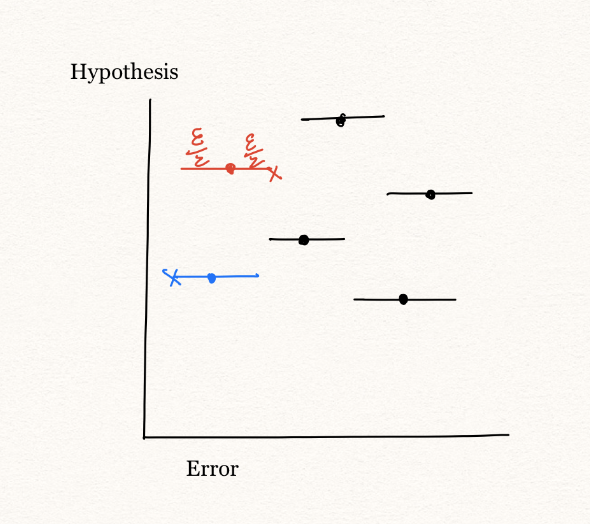
\includegraphics[scale = 0.4]{misc/ex_2.png}
        \caption{Agnostic PAC-learning}
        \label{fig:my_label}
    \end{figure}
The dots are the training error of different hypotheses. Since the sample is $2-\varepsilon$ representative, we know that the true error is within $2-\varepsilon$ of the training error. Our ERM-algorithm will return a hypothesis with minimum training error. In the picture, both the red and the blue hypothesis achieve the minimum training error, so an ERM algorithm choose either one of them. If our ERM algorithm returns the red one. Worst thing that can happen is that its true error (the red cross) is $2-\varepsilon$ higher than its training error, but for the blue hypothesis, the true error (the blue cross) is $2-\varepsilon$ smaller than its training error. However, the true error of the selected hypothesis is still within $\varepsilon$ of the best true error. Expressing in inequalities: for any $h \in \mathcal{H}$:
\begin{equation*}
    \begin{split}
     \operatorname{err}_{D}(h_{D}) &\leq \operatorname{err}_{D}(h_{D})+\frac{\varepsilon}{2}\\
     & \leq \operatorname{err}_{D}(h)+\frac{\varepsilon}{2}\\
     & \leq \operatorname{err}_{D}(h)+\frac{\varepsilon}{2}+\frac{\varepsilon}{2}\\
     & = \operatorname{err}_{D}(h)+\varepsilon
    \end{split}
\end{equation*}
Hence, on an $\frac{\varepsilon}{2}$-representative sample $D$, the $\text{ERM}_{\mathcal{H}}$-rule yields an optimal result. 

\end{enumerate}



% any other appendix sections
\section{Proof of Hoeffding’s Inequality}
\begin{definition}
(Hoeffding's Inequality)
Let $X_{1},...,X_{m}$ be iid random variables such that $a_{i}<X<b_{i}$ with probability $1$. Let $S_{n} = \Sigma_{i=1}^{n}X_{i}$, then for any $t>0$,  
\begin{equation*}
    P(|S_{n} - E[S_{n}]|\geq t) \leq 2e^{- \frac{2t^2}{\Sigma_{i=1}^{n}(b_{i}-a_{i}^{2})}}
\end{equation*}
\end{definition}

\begin{proof}
The key to of this proof is the following upper bound: if $X$ is a random variable with $E[X]=0$ and $a \leq X \leq b,$ then
$$
E\left[e^{s X}\right] \leq e^{\frac{s^{2}(b-a)^{2}}{8}}
$$
To derive the upper bound, by the convexity of the exponential function,
$$
e^{s x} \leq \frac{x-a}{b-a} e^{s b}+\frac{b-x}{b-a} e^{s a}, \text { for } a \leq x \leq b
$$

Therefore,
$$
\begin{aligned}
E\left[e^{s X}\right] & \leq E\left[\frac{X-a}{b-a}\right] e^{s b}+E\left[\frac{b-X}{b-a}\right] e^{s a} \\
&=\frac{b}{b-a} e^{s a}-\frac{a}{b-a} e^{s b}, \text { since } E[X]=0 \\
&=\left(1-\theta+\theta e^{s(b-a)}\right) e^{-\theta s(b-a)}, \text { where } \theta=\frac{-a}{b-a}
\end{aligned}
$$
Now let
$$
u=s(b-a) \text { and define } \phi(u) \equiv-\theta u+\log \left(1-\theta+\theta e^{u}\right)
$$
Then we have
$$
E\left[e^{s X}\right] \leq\left(1-\theta+\theta e^{s(b-a)}\right) e^{-\theta s(b-a)}=e^{\phi(u)}
$$
Using Taylor's expansion:
$$
\phi(u)=\phi(0)+u \phi^{\prime}(0)+\frac{u^{2}}{2} \phi^{\prime \prime}(v) \text { for some } v \in[0, u]
$$

$$
\begin{aligned}
\phi^{\prime}(u) &=-\theta+\frac{\theta e^{u}}{1-\theta+\theta e^{u}} \Rightarrow \phi^{\prime}(u)=0 \\
\phi^{\prime \prime}(u) &=\frac{\theta e^{u}}{1-\theta+\theta e^{u}}\left(1-\frac{\theta e^{u}}{1-\theta+\theta e^{u}}\right) \\
&=\rho(1-\rho)
\end{aligned}
$$
$\mathrm{Now}, \phi^{\prime \prime}(u)$ is maximized by
$$
\rho=\frac{\theta e^{u}}{1-\theta+\theta e^{u}}=\frac{1}{2} \Rightarrow \phi^{\prime \prime}(u) \leq \frac{1}{4}
$$
So,
$$
\begin{aligned}
\phi(u) & \leq \frac{u^{2}}{8}=\frac{s^{2}(b-a)^{2}}{8} \\
\Rightarrow E\left[e^{s X}\right] & \leq e^{\frac{s^{2}(b-a)^{2}}{8}}
\end{aligned}
$$

Now, we can apply this upper bound to derive Hoeffding's inequality.
$$
\begin{aligned}
P\left(S_{n}-E\left[S_{n}\right] \geq t\right) & \leq e^{-s t} \prod_{i=1}^{n} E\left[e^{s\left(L_{i}-E\left[L_{i}\right]\right)}\right] \\
& \leq e^{-s t} \prod_{i=1}^{n} e^{\frac{s^{2}\left(b_{i}-a_{i}\right)^{2}}{8}} \\
&=e^{-s t} e^{s^{2} \sum_{i=1}^{n} \frac{\left(b_{i}-a_{i}\right)^{2}}{8}} \\
&=e^{\frac{-2 t^{2}}{\sum_{i=1}^{n}\left(b_{i}-a_{i}\right)^{2}}} \\
& \text { by choosing } s=\frac{4 t}{\sum_{i=1}^{n}\left(b_{i}-a_{i}\right)^{2}}
\end{aligned}
$$
Similarly, $P\left(E\left[S_{n}\right]-S_{n} \geq t\right) \leq e^{\frac{-2 t^{2}}{\sum_{i=1}^{n}\left(b_{i}-a_{i}\right)^{2}}}$ . This completes the proof of the Hoeffding's theorem. 
\end{proof}

% bibliography
\printbibliography

\end{document}